\paragraph{Testing methods.} The test data is composed of four
distinct datasets:
\begin{enumerate}[A.]
    \item A simulated dataset similar to the training dataset (14 different individuals, 1008 images)
    \item A small annotated set of plants from real Arabidopsis thaliana (4 different individuals, 6 images);
    \item A larger set of real Arabidopsis thaliana for qualitative evaluation (12 different indivudals, 864 images);
    \item A set of real images from another plant (tomato) to evaluate the possibility of transfering the learning onto other species of plants.
\end{enumerate}
All datasets will be available there: TODO.

Evaluation is done both on the 2D segmentation and on the resulting segmented 3D point cloud. For datasets A and B,
we present a class by class quantitative evaluation of the 2D segmentation method. For dataset A, we additionally  provide
class by class quantitative evaluation of the 3D voxel segmentation, as well as a comparison of output point clouds
to the ground truth given by L-Py. For dataset C, we provide qualitative assessment of the results of the segmentation,
both in 2D and in 3D. For dataset D, we restrict ourselves to qualitative evaluation of the 2D segmentation and 3D reconstruction.

Real specimen of Arabidopsis thaliana represent different mutant types and
development stages -- younger or older individuals, with a single or multiple stems -- as can be seen on figure~\ref{fig:realscans}.
Their appearance in pictures are very different from the simulated models
used, such that their segmentation is quite challenging.

The background class is not considered as a class in itself in the evaluation, but is presented in the qualitative example. It
is only used for contrast when reconstructing point cloud from voxel data.

\paragraph{2D Segmentation and 3D Segmentation on dataset A.}
Images from datasets A are segmented used the trained neural network. Then, the results of 2D segmentation are
compared to the ground truth provided by the blender simulation. Figure~\ref{fig:seg2d_res} presents a sample from
dataset A and its segmentation.

\begin{figure}
    \centering 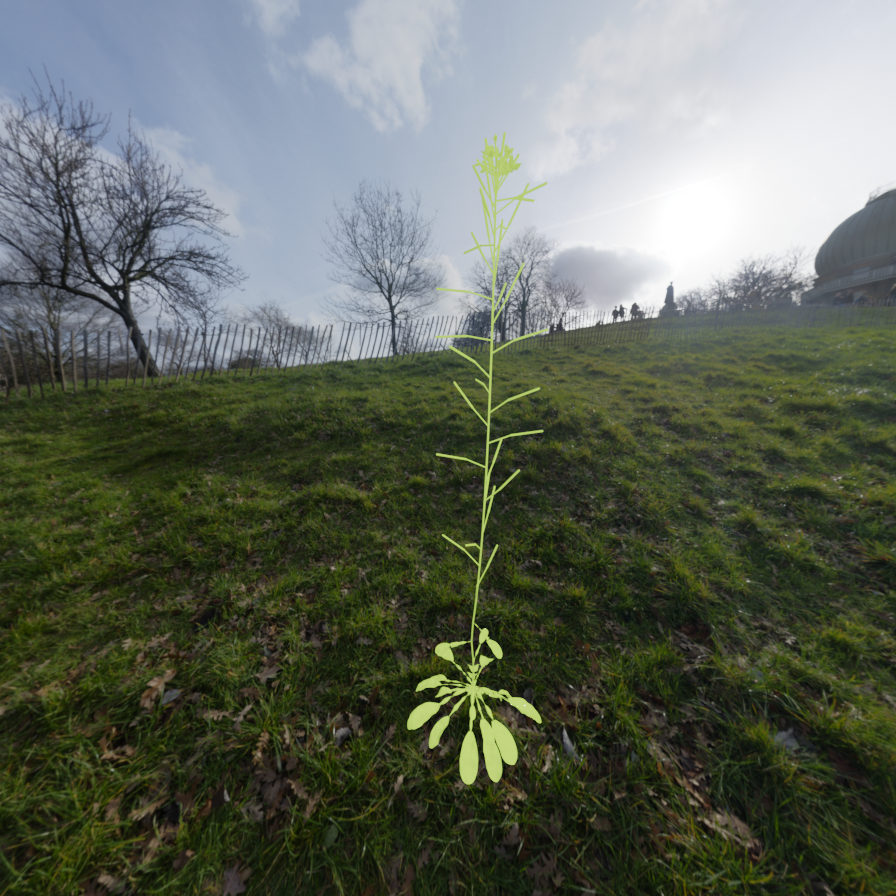
\includegraphics[width = 0.25\linewidth]{figures/00000_rgb.png}\quad
    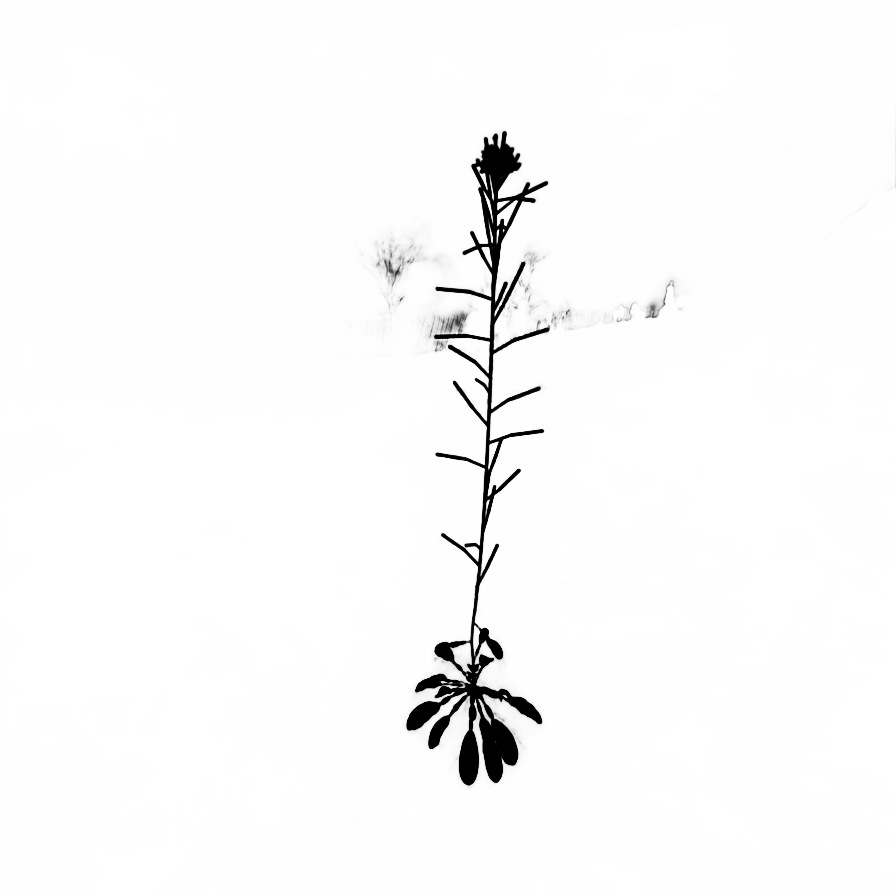
\includegraphics[width = 0.25\linewidth]{figures/000_background.png}\quad
    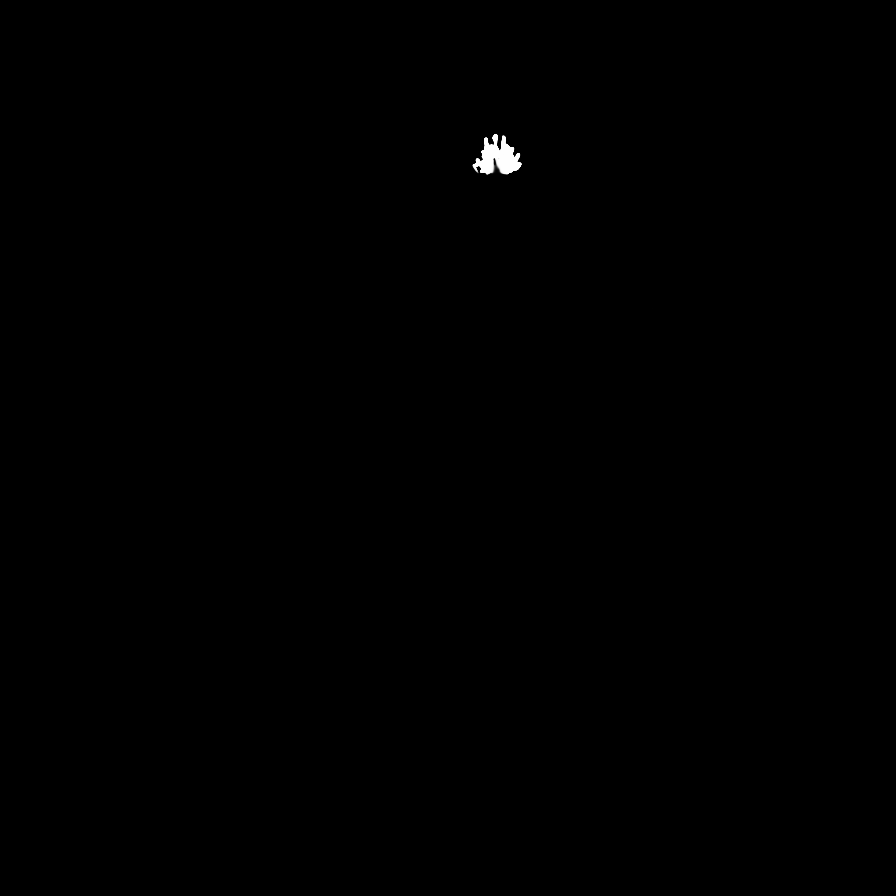
\includegraphics[width = 0.25\linewidth]{figures/000_flower.png}

    \vspace{1em}

    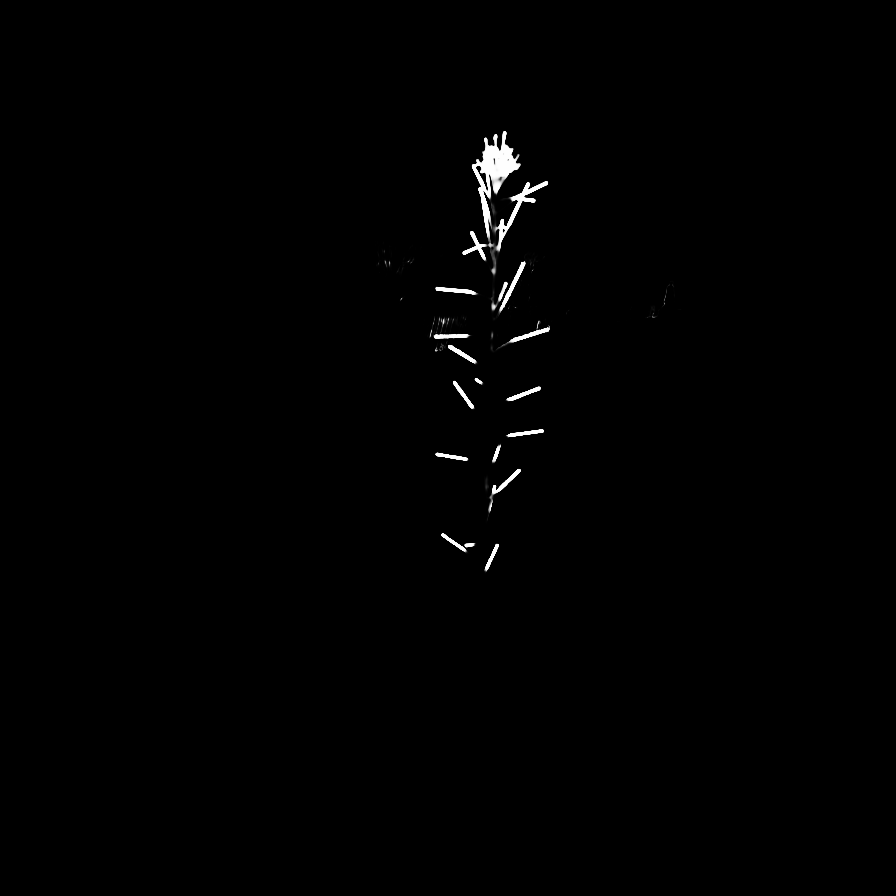
\includegraphics[width = 0.25\linewidth]{figures/000_fruit.png}\quad
    
\includegraphics[width = 0.25\linewidth]{figures/000_leaf.png}\quad
    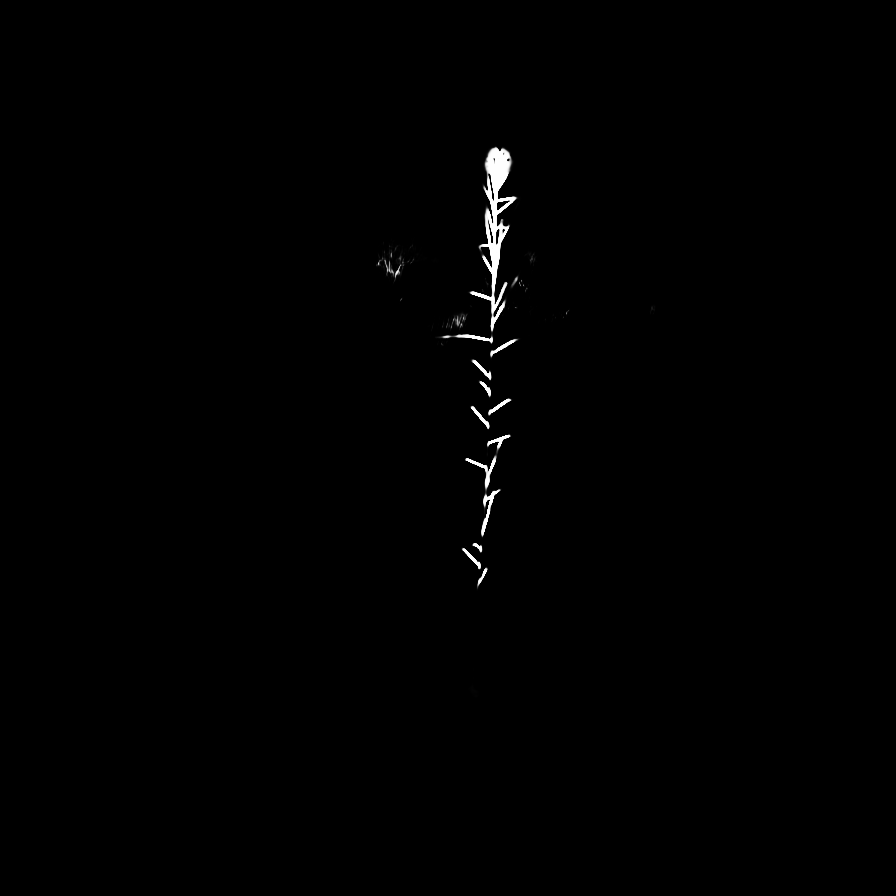
\includegraphics[width = 0.25\linewidth]{figures/000_pedicel.png}
    \caption{Images segmented with our network. From left to right, then top to bottom: original image,
        background, flower, fruit, leaf, pedicel. White indicates a high score (1.0) for the class,
        black indicates a low score (0.0).} \label{fig:seg2d_res}
\end{figure}

Pixels are classified using a threshold on the output of the segmentation
network: for each class $k$, if the score of a pixel is $>0.5$, then the pixel is
positively attributed to class $k$. Given the high contrast of the output images
from the neural netork, the chosen threshold does not matter much. Every pixel
$x$ in then attributed to one of four sets, as classical in the litterature:

\begin{itemize}
    \item $x$ belongs to $\textrm{TP}$ (true positive) if our predicted class is positive and the actual class is
positive;
    \item $x$ belongs to $\textrm{TN}$ (true negative) if our predicted class is negative and the actual class is
negative;
    \item $x$ belongs to $\textrm{FP}$ (false positive) if our predicted class is positive and the actual class is
negative;
    \item $x$ belongs to $\textrm{FN}$ (false negative) if our predicted class is negative and the actual class is
positive;
\end{itemize}

For voxels, the same classification is applied and each voxel is attributed a single class
from the segmentation algorithm presented above, and its class is compared to
the class of the closest point on the mesh produced by L-py.

For both pixels, and voxels, precision and recall are defined as follows and
used as a metric for the accuracy of segmentation:

$$
    \textrm{precision} = \frac{\textrm{\# TP} }{\textrm{\# TP} + \textrm{\# FP}},
    \textrm{recall} = \frac{\textrm{\# TP} }{\textrm{\# TP} + \textrm{\# FN}},
$$

Precision is the proportion of the predicted class which is correctly labeled,
recall is the proportion of all elements of a class which have been predicted.
Figure~\ref{fig:prec_recall_2d_3d} present precision and recall for each class
for both 2D and 3D segmentation. Voxels and pixels are accumulated over all of
dataset A. \\
The results show that the precision for each class is higher in 3D than in 2D. This is because the transfer to 3D reduces the number of false positives. Two reasons explainin the presence of false-positive in the 2D segmented images. First, the 3D reconstruction carves away the voxels based on the prediction of pixels onto they project. Therefore to avoid losing voxels that are part of the plant, we prefer  to favor false-positive against false-negatives on the 2D predictions and keep a low threshold to make the prediction masks. Second, the network is trained to predict overlaps of classes: one pixel can be attributed to multiple classes. This also favors false-positives over false-negatives. As stem, pedicel and fruits have similar structures (thin and elongated), the segmentation network tends to mix-up the classes and overlap predictions of these classes. However, when projecting in 3D only one class can be attributed per voxel. This class is the most probable class from all viewpoints, which allows to reduce the number of misattributions. On the other hand the first step of the 3D reconstruction consists in carving away all the voxels that are not belonging to the plant. If some pixels that were in the plant are removed in this step, it is impossible to recover them. Therefore the number of false negative increases in the 3D step, which has effect on the recall. This happens for the stem which is sometimes discontinuously reconstructed due to error of prediction on the background class. The false negatives also come from misattribution of class. For example the flowers are very thin, small and surrounded by other organs which makes them hard to predict precisely. It is also significant at organ intersections, for example where the pedicel are branched to the stem. 

\begin{figure}[h!]
    \centering 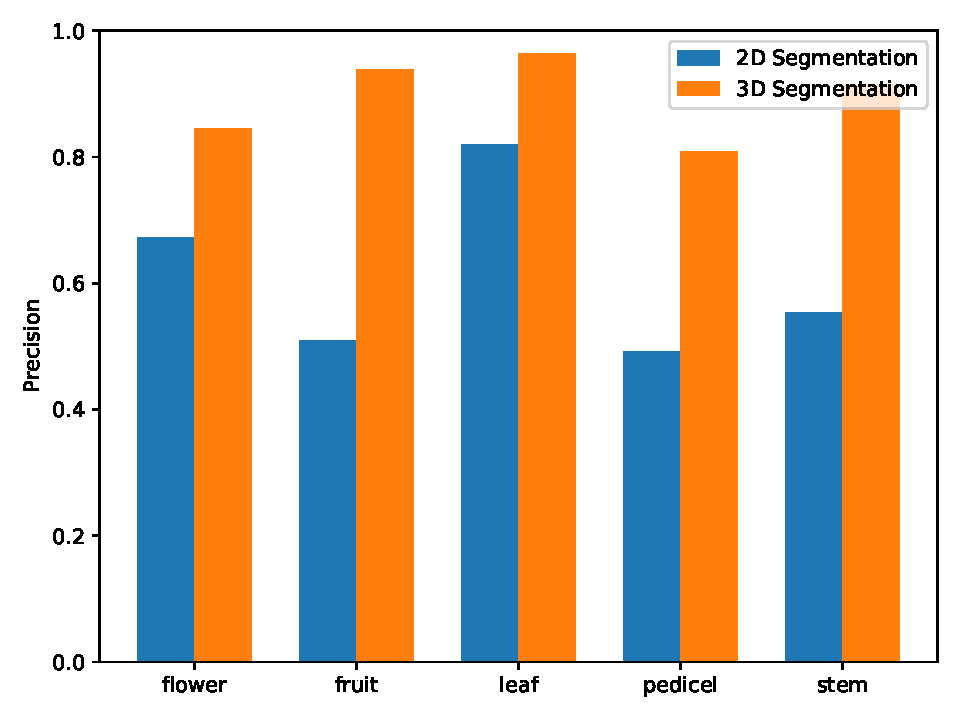
\includegraphics[width = 0.5\linewidth]{figures/eval_precision.pdf}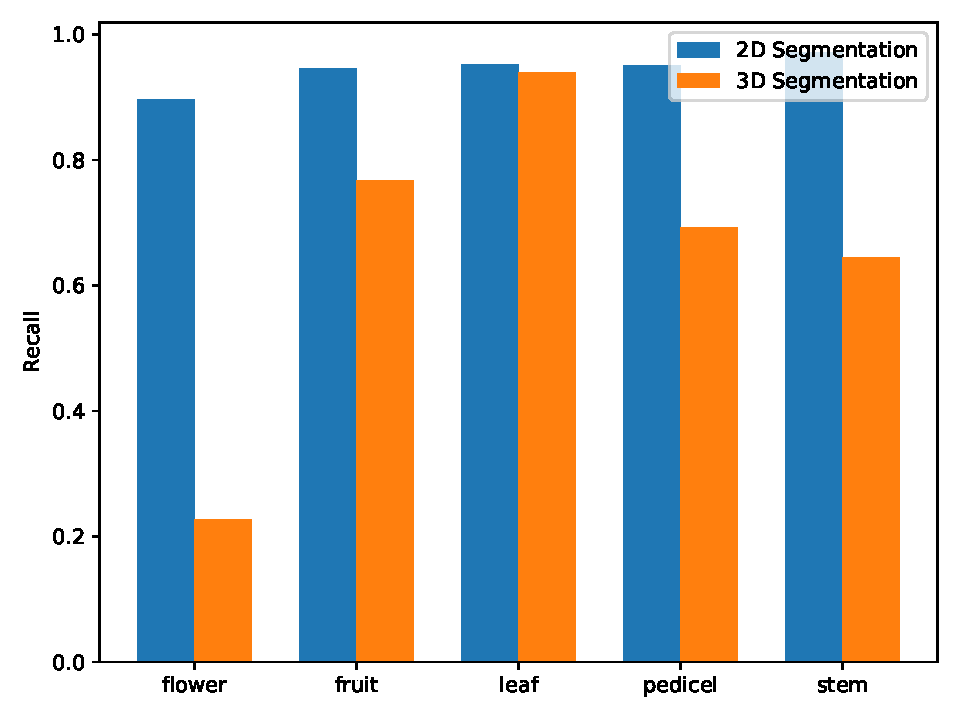
\includegraphics[width = 0.5\linewidth]{figures/eval_recall.pdf}
    \caption{Precision and recall comparison between 2D segmentation and 3D
segmentation.} \label{fig:prec_recall_2d_3d}
\end{figure}


\paragraph{2D Segmentation of real arabidopsis.}
 We then manually annotated real images of \emph{A. Thaliana} (dataset B) and evaluated the performance of the model trained on the virtual dataset. We present precision and recall results for each class, comparing results on virtual plants and real plants (Figure \ref{fig:prec_recall_virt_real}). It has to be noted that the size of the dataset (6 pictures) is small and limiting for proper statistical analysis. Although the network makes more errors than with the virtual plants, we get satisfactory segmentation results. Among the errors, mix-up between the stem, fruit and pedicel classes is more present and the network has difficulties distinguishing fruits and leaves when they grow along the setm. Observing the errors made by the network allowed us to improve the 3D models of the plants based on the errors the segmentation was making: we included rotation of the leaves, bending of the stem and random coloration of the organs. This allowed to both improve the plant models and the 2D-segmentation network. Overall, the 3D models of the plant and the images generated in the virtual environment are good enough to obtain a satisfactory segmentation of the plants and especially on the 3D reconstruction of the real plants.\\


\begin{figure}[h!]
    \centering 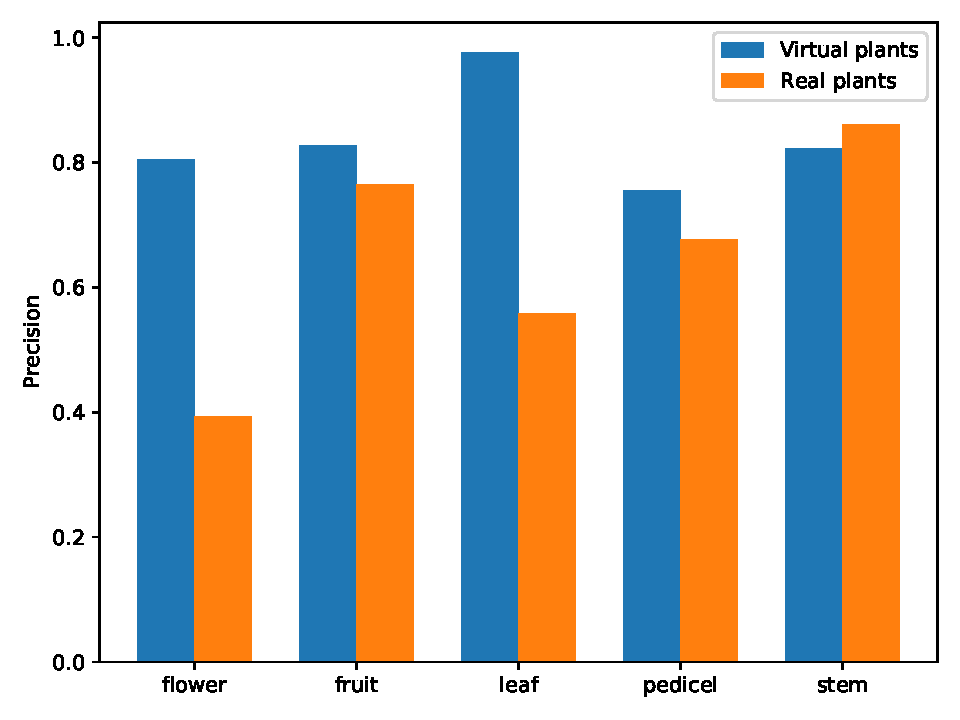
\includegraphics[width =
0.5\linewidth]{figures/eval_precision_real.pdf}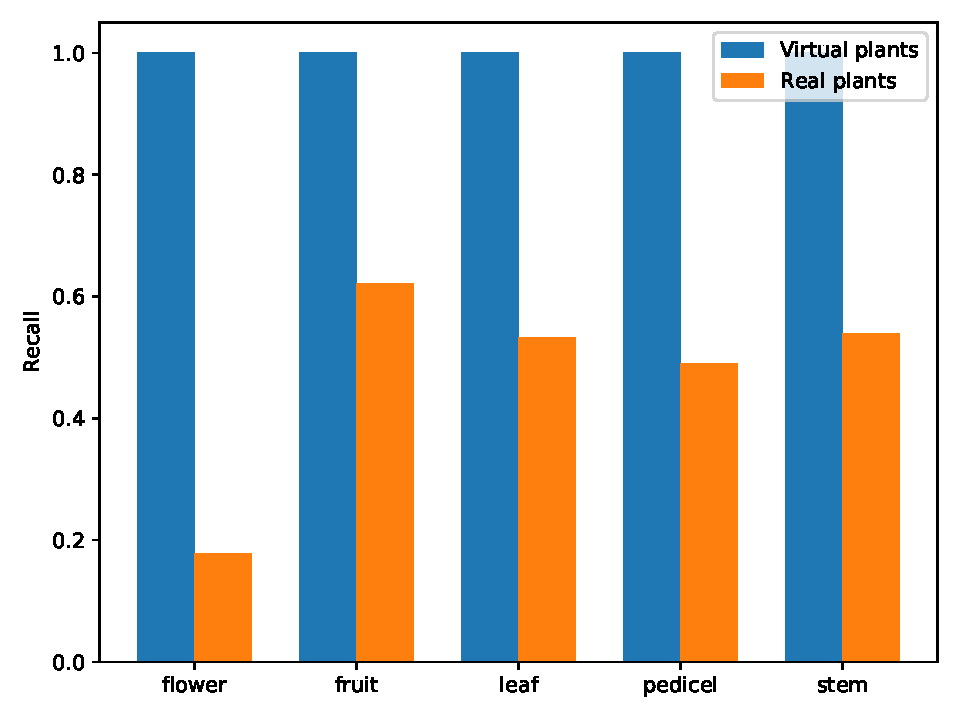
\includegraphics[width =
0.5\linewidth]{figures/eval_recall_real.pdf}
    \caption{Precision and recall comparison between 2D segmentation on
virtual and real images unseen by the neural network.} \label{fig:prec_recall_virt_real}
\end{figure}

\paragraph{Qualitative evaluation on real plants.}
We then segmented and reconstructed  \emph{A. Thaliana} real plants from dataset C. Some example pictures are shown on Figure \ref{fig:realscans}. Without ground truths we can only give a qualitative analysis of the results (Figure \ref{fig:rec3d}). The reconstructions and segmentation were qualitatively as good as the 3D reconstruction to the point where in some cases it is hard to tell whether the reconstructed plant is from a real or a virtual plant. One default is that the reconstruction of the leaves at the basis on the stem is not accurate. This is due to the fact that these leaves are hardly identifiable, mixed with the pot or dried out. They are of little phenotypical interest so we didn't focus on solving this issue. Another issue comes from occlusions, especially of the stem. The reconstruction fails for example when there are several plants grouped together in ths same pot, or when there is a structure unknown to the segmentation network, for example a tutor obstructing some viewpoints. To solve the first issue one solution would be to increase the variety in the viewpoints, by taking pictures from the top of the pot. To solve the second, we would need to teach the network to interpret occlusions by foreign objects, by including such objects in the virtual scene for example.

\begin{figure}[h!]
    \centering 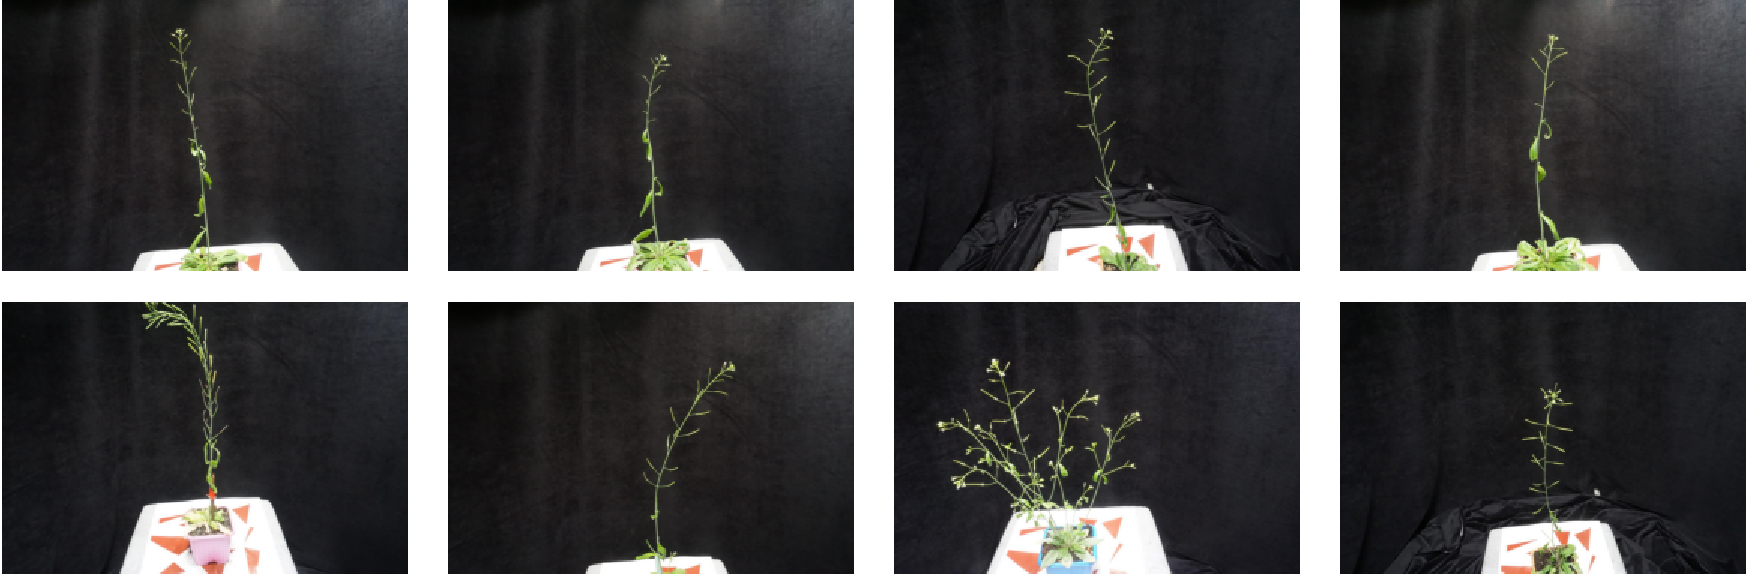
\includegraphics[width = \linewidth]{figures/seg-crop.pdf}
    \caption{Sample images from the dataset used for qualitative assessment of the method on real data} \label{fig:realscans}
\end{figure}

\begin{figure}[h!]
    \centering 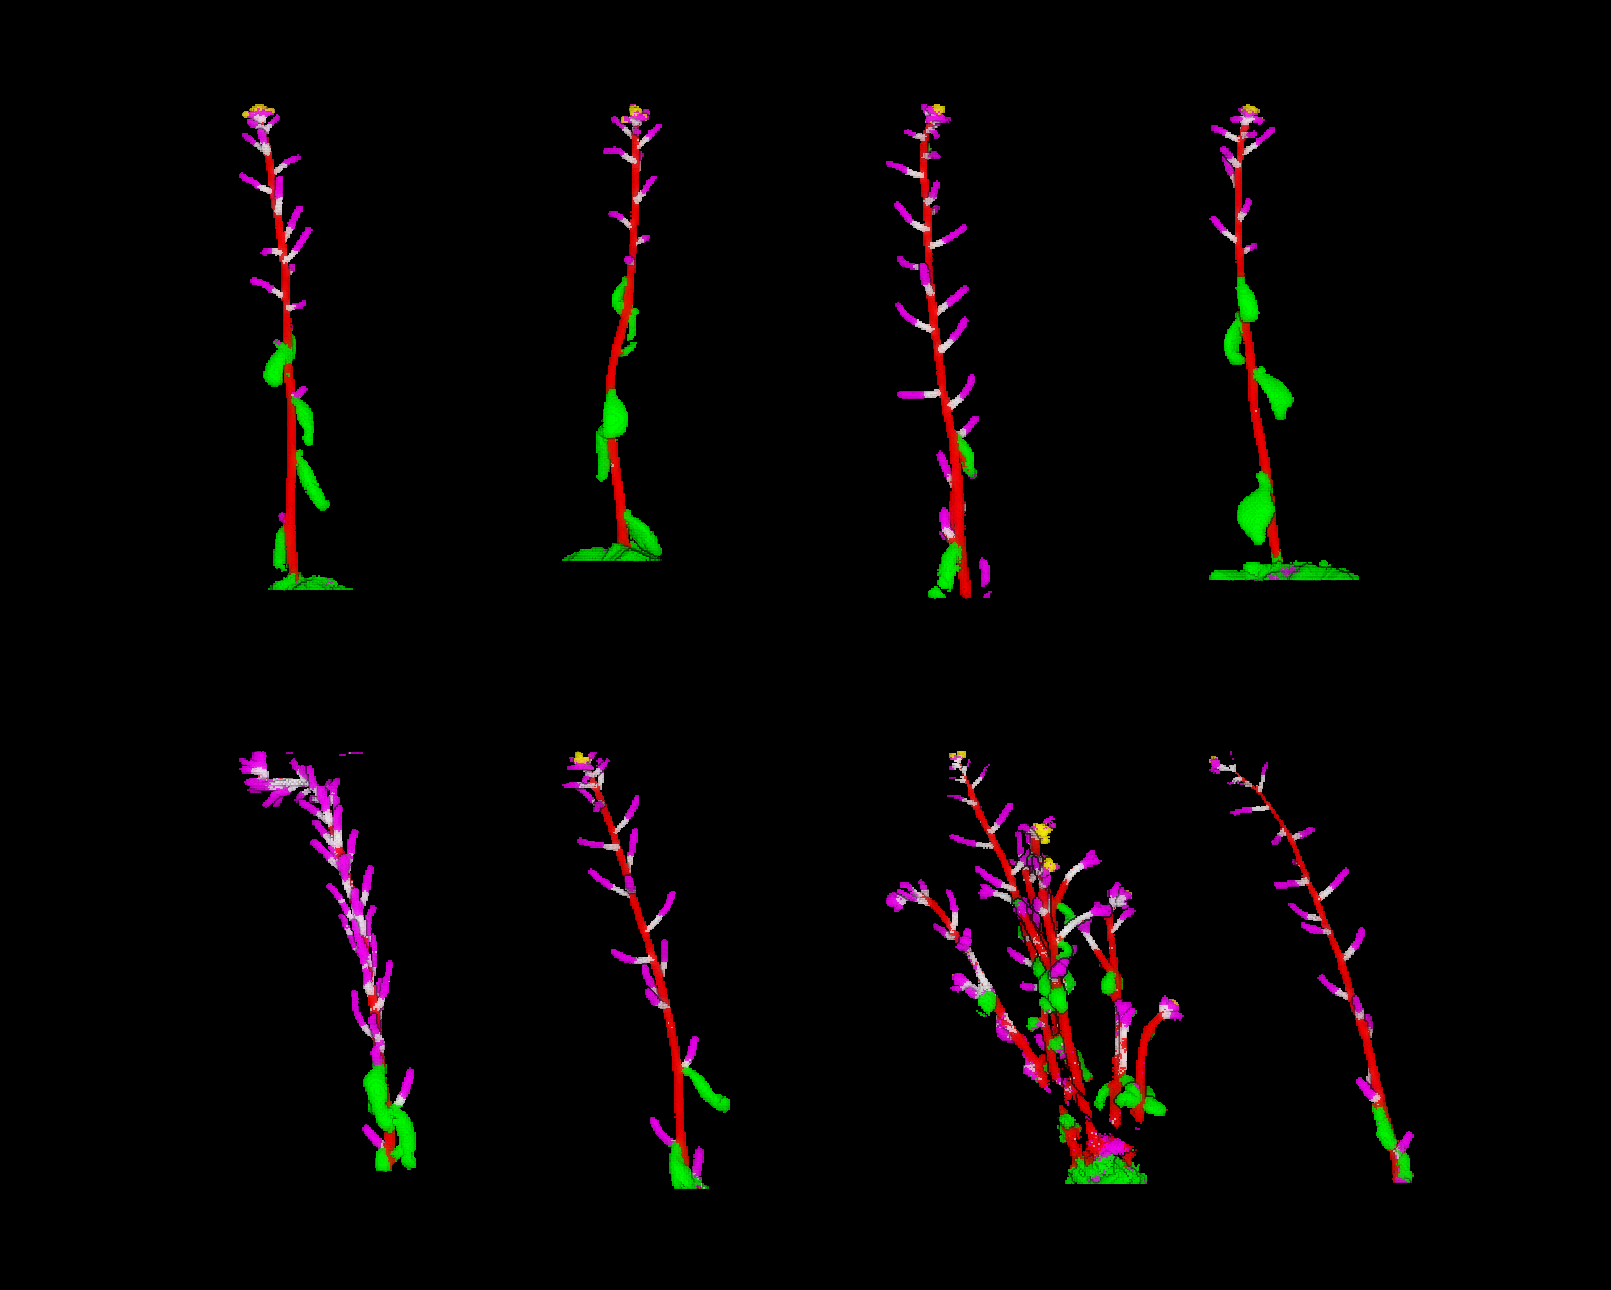
\includegraphics[width = 0.7\linewidth]{figures/capture.png}
    \caption{3D reconstruction of real plants. Red: stem, green: leaf, white: pedicel, purple: fruit:, yellow: flower} \label{fig:rec3d}
\end{figure}

\paragraph{Transfer to other species.}
To transfer to species anatomically different from \emph{A. Thaliana} we used model finetuning. This step requires a minimal number of manually annotated images (2 or 3) of the other species and allows to reconstruct the full model in 3D. To test the finetuning method we took a video turning around a tomato plant and sampled 41 images equally distributed along the video to get images from different viewpoints. Then 2 images were manually annotated with our interface. We included only the two classes present: stem and leaf. Then the network trainied on virtual \emph{A. Thaliana} was trained on these two images for 20 epochs. Then we ran the 2D segmentation (Figure \ref{fig:finetune2D}) 3D reconstruction pipeline and obtained a 3D model of the tomato (Figure \ref{fig:finetune3D}). We notice that the reconstruction of the plant at the level encompassed properly in the field of view of the camera is correct. However the top leaves reconstruction suffers from lack of information. To improve the quality of the reconstruction more points of view of the tomatoe would have been needed. 

\begin{figure}[h!]
    \centering 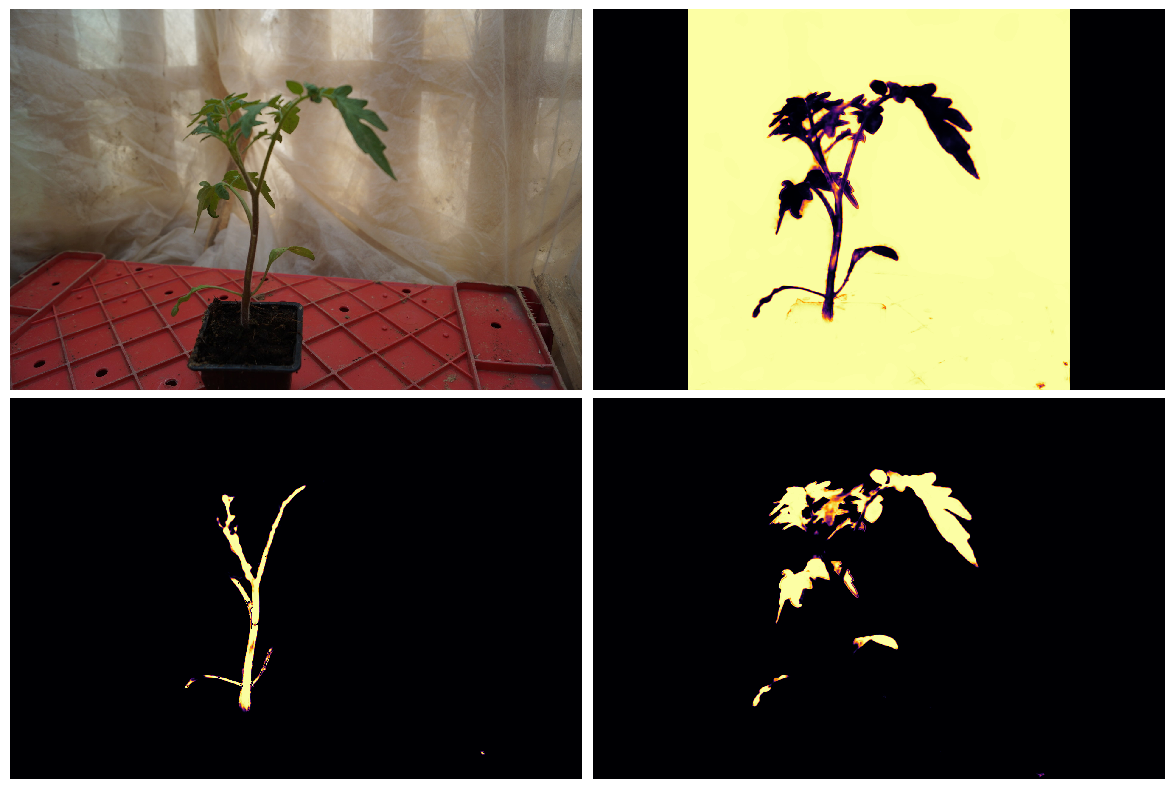
\includegraphics[width = \linewidth]{figures/finetune.png}
    \caption{Predictions of the model finetuned on two images of tomato manually annotated. (The masks of pedicel and stem are superimposed on this figure but they were predicted separately).} \label{fig:finetune2D}
\end{figure}


\begin{figure}[h!]
    \centering 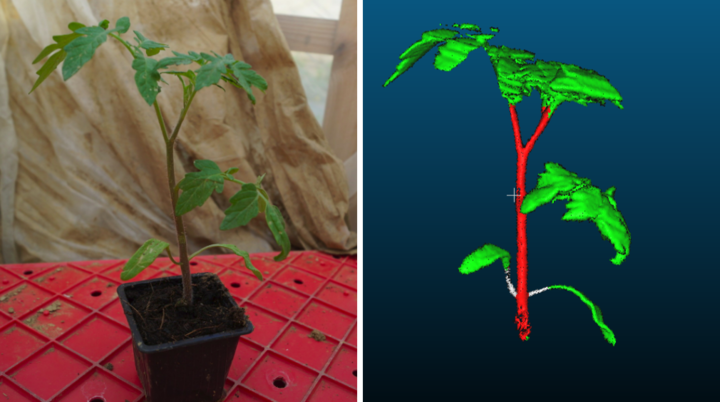
\includegraphics[width = \linewidth]{figures/tomato.png}
    \caption{3D reconstruction and segmentation of tomato plant with the pipeline.} \label{fig:finetune3D}
\end{figure}


